% !TEX root = thesis-thomas-tiotto.tex
\todo{introduzione con outline del capitolo}
\todo{riassunto della fine del capitolo}

\section{Mathematical Background}
Bayesian Networks (BN) are a class of Probabilistic Graphical Models that are used to represent systems under conditions of uncertainty.
To give a formal definition we will first need a few basic concepts from probability and graph theory.

\subsection{Probability Theory}
\subsubsection{Probability distributions}
\begin{definition}
	A \textit{probability distribution} is a function $\mathbb{P}: \mathcal{S} \rightarrow \mathbb{R}$ with $\mathcal{S}$ a set of \textit{events} of interest.  
To be a valid probability distribution $\mathbb{P}$ must satisfy:
\begin{itemize}
	\item $\mathbb{P}(\sigma) \geq 0 \quad \forall \sigma \in \mathcal{S}$
	\item $\sum_{\sigma} = 1 \quad \forall \sigma \in \mathcal{S}$
	\item $\alpha, \beta \in \mathcal{S} \wedge \alpha \cap \beta=\emptyset 	\Rightarrow \mathbb{P}(\alpha \cup \beta)=\mathbb{P}(\alpha)+\mathbb{P}(\beta)$
\end{itemize}
\end{definition}
Each event $\sigma \in \mathcal{S}$ must have a probability $\mathbb{P}(\sigma) \in [0,1]$ and the sum of all these must equal $1$. 
An event with $P(\sigma) = 0$ is deemed \textit{impossible} while one with $\mathbb{P}(\sigma) = 1$ is \textit{certain}.

There is some discord regarding how to actually \textit{interpret} the probability of an event.
What I believe to be the initially commonly held view is the \textit{frequentist} one, that views the probability of an event as the ratio of times it would occur over a great number of trials.  
So, for example, saying that obtaining a heads has probability $0.5$ when tossing a coin would mean that over repeated throws we would observe heads half the time.

Another, commonly held view is the \textit{Bayesian} (from the 18th century mathematician Thomas Bayes) one in which probabilities are viewed as the \textit{subjective} degree of belief attributable regarding the manifestation of an event.
In this interpretation, stating that a coin has $0.5$ probability of landing on heads simply means that the person making the claim personally believes that the chances of seeing heads of tails are the same.
This is obviously a ``softer'' definition compared to the frequentist one but it is nonetheless useful in that it lets one characterise certain events that haven't come about yet or are liable to happen only once or a few times.

Philosophically, Bayesian inference assigns a probability to a hypothesis (a \textit{prior}) while the frequentist method tests a raw hypothesis empirically before assigning it any probability.
As Bayesian inference naturally embraces and deals with uncertainty, it is an enormously useful tool to model and reason about the real, stochastic world we live in.

\subsubsection{Random Variables}
\begin{definition}
	A random variable is a function that associates every outcome in $\mathcal{S}$ with a value.
\end{definition}
\textit{Random variables} are a way of bringing to the fore the attributes of interest of events while dealing with them in a clean, mathematical way.
The values that a random variable can take are a function of the events in sample space $\mathcal{S}$, each of these is assigned a value by the random variable function.
I will only be dealing with \textit{categorical random variables} i.e. those who's codomain is a discrete set of values.
Every random variable has a probability distribution induced by the cardinality of the subsets of its values; in the case of categorical-valued one, such a distribution is \textit{multinomial}.

If we were to take a Bayesian point of view, we would consider a random variable as simply representing the subjective degree of belief we would have over a set of outcomes we believed possible.

\subsubsection{Conditional Probabilities}
After having defined the basic notion of probability, we can construe one the basic building blocks of Bayesian Networks: the concept of \textit{conditional probability} 
\begin{definition}
	The conditional probability, ``the probability of event $\beta$ given event $\alpha$'' is:
\begin{equation} \label{eq:conditionalprobability}
\mathbb{P}(\beta \mid \alpha) = \frac{\mathbb{P}(\beta \cap \alpha)}{\mathbb{P}(\alpha)}
\end{equation}
\end{definition}
That is, the relative proportion of event $\beta$ compared to event $\alpha$; this intuitively represents the probability of $\beta$ \textit{knowing} that $\alpha$ has already occurred.

Equation \ref{eq:conditionalprobability} can be easily manipulated to obtain another basic element of Bayesian Networks: what is called the \textit{chain rule of conditional probabilities}:
\begin{equation} \label{eq:chainrule}
	\mathbb{P}(\beta \cap \alpha) = \mathbb{P}(\beta \mid \alpha) \mathbb{P}(\alpha)
\end{equation}
This can be generalised to any number of events:
\begin{equation} \label{eq:chainrule}
	\mathbb{P}(\alpha_1 \cap \ldots \cap \alpha_n) = \mathbb{P}(\alpha_n \mid \alpha_1 \cap \ldots \cap \alpha_{n-1}) \ldots \mathbb{P}(\alpha_1 \mid \alpha_2 ) \mathbb{P}(\alpha_1) 
\end{equation}
Intuitively, it means that we can decompose joint probabilities as products of conditional probabilities.  
As we'll see, this is how the values in a Bayesian Network are calculated.

\subsubsection{Independence}
Now, we have just seen in Equation \ref{eq:conditionalprobability} that, in general, $\mathbb{P}(\beta | \alpha) \neq \mathbb{P}(\alpha)$ because $\mathbb{P}(\beta \cap \alpha) \neq \mathbb{P}(\beta) \mathbb{P}(\alpha)$
\begin{definition}
Two events $\alpha$ and $\beta$ are \textit{unconditionally independent} $A \perp B$ - or simply \textit{independent} - when:
\begin{equation}
	\mathbb{P}(\beta \mid \alpha) = \mathbb{P}(\beta) \Leftrightarrow \beta \perp \alpha
\end{equation}
\end{definition}
This means that knowing that $\alpha$ took place doesn't change our beliefs around $\beta$ happening. 
In the real world it is hard, or actually impossible if we consider existence at a fine-enough level to involve Chaos Theory, to find two such perfectly non-interacting events.
Thus, a more useful concept is that of \textit{conditional independence} where two previously dependent event become independent when also conditioned on a third one.
\begin{definition}
Two events $\alpha$ and $\beta$ are \textit{conditionally independent} $(\beta \perp \alpha \mid \gamma)$ when:
	\begin{equation}
	\mathbb{P}(\beta \mid \alpha \cap \gamma ) = \mathbb{P}(\beta \mid \gamma) \Leftrightarrow (\beta \perp \alpha \mid \gamma)
\end{equation}
\end{definition}

\subsubsection{Correlation}
Correlation, as defined by \cite{Stolp2006}, is a measure of the degree to which two random variables are linearly dependent.
The most used measure of such a dependence is the \textit{Pearson Correlation Coefficient} or \textit{bivariate correlation}.
\begin{definition}
	The correlation coefficient $\rho$ of random variables $X$ and $Y$ is given by:
	\begin{align} \label{eq:correlation}
		\rho_{XY} &= \frac{Cov(X,Y)}{\sigma_X \sigma_Y} \\
		&= \frac{\mathbb{E}[ (X - \mu_X) (Y - \mu_Y) ]}{\sigma_X \sigma_Y} \\
		&= \frac{\sum_{x \in \mathcal{X}} \sum_{y \in \mathcal{Y}} (x - \mu_X) (y - \mu_Y) p_{XY}(x,y)}{ \sqrt{\sum_{x \in \mathcal{X}}  (x - \mu_X)^2 p_X(x)} \sqrt{\sum_{y \in \mathcal{Y}} (x - \mu_Y)^2 p_Y(y)} } 
	\end{align}
	with $p_{XY}$ the joint probability mass function of $X$ and $Y$ and $p_{X}$ and $p_{Y}$ the marginal distributions of $X$ and $Y$, respectively.
\end{definition}
That is, the bivariate correlation coefficient for random variables $X$ and $Y$ is given by the \textit{covariance} of $X$ and $Y$ divided by the product of their standard deviations.

The covariance is the \textit{first centred moment} of the \textit{joint distribution} of $X$ and $Y$ while the \textit{standard deviation} is the square root of the \textit{second centred moment} of the marginals.

$\rho_{XY}$ is normalised so its values vary in the interval $[-1,1]$; the correlation coefficient represents the degree of linear association between the two variables with $\rho_{XY}=-1$ being called \textit{perfect anticorrelation} and $\rho_{XY}=+1$ \textit{perfect correlation}.
The two correspond to the cases where the linear equation perfectly describes the relationship between $X$ and $Y$; the sign indicates the slope of the regression line describing the relationship i.e. if an increase in one of the two variables corresponds to an increase in the other in the pair, or viceversa.
The closer $\rho_{XY}$ tends to $0$, the feebler the relationship between $X$ and $Y$ with the case $\rho_{XY}=0$ indicating that the two variables are \textit{independent}.

\subsubsection{Mutual Information} \label{subsec:mutualinformation}
Another way of characterising the interrelatedness of two variables is through the concept of \textit{mutual information}, as defined in \cite{Cover2006}, that is closely linked to entropy, see Eq. \ref{eq:entropy}.
\begin{definition}
	The mutual information of two random variables $X$ and $Y$ is given by:
	\begin{equation}
		I_{XY} = \sum_{x \in \mathcal{X}} \sum_{y \in \mathcal{Y}} p_{XY}(x,y) \log \left( \frac{p_{XY}(x, y)}{p_{X}(x) p_{Y}(y)} \right)
	\end{equation}
\end{definition}
$I_{XY}$, intuitively, measures the amount of information that $X$ and $Y$ share that can also be seen as the degree to which one variable is informative of the other.
If $X$ and $Y$ are independent then they share no mutual information and knowing one of the two gives no information about the other.
if $X$ and $Y$ are perfectly correlated ($\rho_{XY}= \pm 1$) then they both convey the same amount of information and $I_{XY}$ is equal to the entropy $\Eta(X) = \Eta(Y)$.

\subsection{Information Theory} \label{subsec:information-theory}
The birth of the field of \textit{information theory} is usually traced back to the seminal paper \enquote{A Mathematical Theory of Communication} (\cite{Shannon1949}) where Claude Shannon set the mathematical basis for the quantification of the amount of \textit{information} transmissible over a noisy channel. 
In his words \enquote{The fundamental problem of communication is that of reproducing at one point, either exactly or approximately, a message selected at another point.}
The concepts of field are broad enough to have influenced practically every other scientific discipline and deep enough to have enabled the \enquote{digital age}, for example by enabling the creation of ever more complicated coding schemes for the compression, reconstruction and obfuscation of digital data.

\subsubsection{Entropy}
In classical mechanical statistics, entropy can be seen as a measure of the uncertainty, or randomness, of a physical system.  
This concept was reapplied by Shannon to measure the amount of randomness in a random variable.
\begin{definition}
	Given a random variable $X$ with probability distribution $\mathbb{P}(X)$, its entropy $\Eta(X)$ is defined as the expected amount of information content carried by $X$ (\cite{Schneider2005}):
\begin{equation} \label{eq:entropy}
	\Eta(X) = \mathbb{E}(I(X)) = \mathbb{E}(-\log (\mathbb{P}(X)) = -\sum_{i=1}^{n} \mathrm{P}\left(x_{i}\right) \log _{b} \mathrm{P}\left(x_{i}\right)
\end{equation}
\end{definition}
The base $b$ of the logarithm defines the unit of measure.  Shannon used $b=2$ as he was dealing with the transmission of digital, binary-coded data; in this case the unit of measure are $bits$.

The simplest example of how information entropy characterises a random variable $X$, is in imagining $X$ to model a coin and the task being to predict the probability of the outcome of a throw being heads.
If the coin is fair, we will not be any more surprised to see the outcome being heads than tails; the entropy is maximum as there is maximum uncertainty regarding the outcome.
However, if the coin is not fair and tails is more probable the we will be more surprised than not to see the outcome being heads.  
The entropy is sub-maximal because there is less uncertainty regarding the outcome: tails is more probable than heads.
If one of the outcomes is impossible, for example if the coin has two heads, then the entropy of the coin is $0$ as there is no uncertainty regarding the result of a toss.


\subsubsection{Normalised Entropy}
Plain entropy is not a good choice when trying to characterise random variables with different cardinalities of their sample space.
Let us suppose that the objective is to find the variable with the least \enquote{entropic} distribution and we suppose that their values have all been generated by the same process, say Gaussian.
Simply calculating their entropies and ordering them according to this criterion will bias the selection process towards the variables with smallest cardinality.
This is because we supposed them to be distributed in the same way so there will naturally be less uncertainty when there are fewer possible outcomes.
This can easily be understood by imagining the distributions to all be random uniform.

To obviate to this problem we need to \textit{normalise} the entropy so that different-sized variables can be directly compared to each other.
To achieve this, we can look at a measure of \textit{normalised entropy} or \textit{efficiency}:
\begin{equation} \label{eq:normalisedentropy}
 	\eta(X)=-\sum_{i=1}^{n} \frac{p\left(x_{i}\right) \log _{b}\left(p\left(x_{i}\right)\right)}{\log _{b}(n)}
\end{equation}
From Eq. \ref{eq:normalisedentropy} it can be seen that $\eta(X) \in [0,1]$; it is thus normalised and comparable among distributions.
This ratio expresses the amount of entropy found in the distribution compared to the maximum possible entropy when using $n$ symbols, corresponding to the uniform distribution:
\begin{equation}
\mathrm{H}\left(\underbrace{\frac{1}{n}, \ldots, \frac{1}{n}}_{n}\right) = - \sum_{i=1}^n \frac{1}{n} \log _{b} \left( \frac{1}{n} \right) = -n \cdot \frac{1}{n} \log _{b} \left( \frac{1}{n} \right) = - \log _{b} \left( \frac{1}{n} \right) = \log _{b}(n) 
\end{equation}   

\subsection{Graph Theory} \label{subsec:graph-theory}
Many problems in Machine Learning (ML) don't involve classification or prediction of single data points in isolation, but of set of entities that may present a more, or less, complex relation with each other. 
Most real-world phenomena fit into the latter framework.
Graphs are one of the most powerful tools for the modelling of this class of problems, as their structure naturally captures the wide variety of relations that may exist between entities.
These range from the atomical structure of a molecule to a social network of friends.  
In both these examples graphs help in reasoning, visualising and making inferences and predictions.

\subsubsection{Graphs} 
\begin{definition}
	A graph is a tuple 
	\begin{equation}
	\mathcal{G} = (\mathcal{V}, \mathcal{E})
\end{equation}
with $\mathcal{V} = \{ v_1 \ldots v_n \}$ the set of \textit{vertices} and $\mathcal{E} = \mathcal{V} \times \mathcal{V}$ the set of \textit{edges}.
\end{definition}

For our scopes, we will only be considering the case where every element in $\mathcal{E}$ is a pair either of the form $(v_i, v_j)$ or $(v_j, v_i)$ with $i \neq j$.  
That is to say that the class of graphs presently of interest for us are those where there can be at most a single directed edge between any node in $\mathcal{V}$ and no self-loops.
We are also interested in enforcing that there be no \textit{cycles} in the graph, i.e. sequences of nodes of the form $v_i \rightarrow v_j \rightarrow \cdots \rightarrow v_i$.
The resulting graph possessing only directed edges and no cycles is commonly called a \textit{directed acyclic graph}, or DAG for short.  
This data structure is of paramount importance as it's the fundamental graphical representation used for Bayesian Networks.

\subsubsection{Polytrees}
We now have all elements to be able to formally define a Bayesian Network.
I will also define polytrees and trees because these are a fundamental concept for the work carried out in this thesis.
\begin{definition}
	A \textit{loop} is a trace $v_i, v_j \ldots v_i$ of nodes obtained by following edges regardless of their direction
\end{definition}
\begin{definition}
	A directed graph containing no such loops is called a \textit{polytree}. 
\end{definition}
\begin{definition}
	A \textit{tree} is a particular case of polytree where each node has at most one parent.	
\end{definition}

\subsubsection{D-separation} \label{subsec:d-separation}
\textit{Dependence-separation} or \textit{d-separation}, as the name entails, is a concept relating to the conditional dependence between variables.
It was first presented by \cite{Pearl1988}
To define it, we first have to clarify when two sets of nodes $X$ and $Y$ are causally connected.
This is so if $Z = \emptyset$ and they are part of one of the following three structures, called \textit{v-structures} in this context:
\begin{itemize}
  \item $X \rightarrow Z \rightarrow Y$
  \item $X \leftarrow Z \leftarrow Y$
  \item $X \leftarrow Z \rightarrow Y$
\end{itemize}
This means that knowing something about $X$ also tells us something new about $Y$.
$X$ and $Y$ are causally independent if they appear in the following v-structure:
\begin{itemize}
  \item $X \rightarrow Z \leftarrow  Y$
\end{itemize}
Such a configuration is called a \textit{collider} and it blocks the flow of information from $X$ to $Y$.
If $Z \neq \emptyset$ the cases are reversed so colliders are open and the other three structures are blocked.
\begin{definition}
	Given disjoint subsets $X, Y, Z \subset \mathcal{X}$, $X$ and $Y$ are d-separated if:
	\begin{itemize}
		\item $Z \neq \emptyset$: no path between $X$ and $Y$ presents a collider
		\item $Z = \emptyset$: there is a collider on every path between $X$ and $Y$
	\end{itemize}
\end{definition}

The independencies between variables are encoded in the structure of the DAG so every distribution whose BN has the same connections between nodes also has the same independencies, regardless of the values of the variables.

An example using on the real network used in this thesis is shown in Fig. \ref{fig:d-separation_example}.
Here we can see how the network's topology and the nodes chosen to be in the observed set $Z$ define the resulting separations.
In this case $X= \{ \text{mut17q21} \}$, $Z= \{ \text{differenziazione, pN} \}$ and $Y=V \smallsetminus X \smallsetminus Z$; the resulting set of nodes that are d-separated from $X$ contains $\{ \text{c erB 2, FISH, loss 17, situ, pT, M, lateralita} \}$.
Basically, we are asking for the set of all nodes in the DAG that are d-separated from $X$, given evidence $Z$.
The reason for this can easily be given by enumerating all paths through the v-structures in the network and applying the definitions for causal connections given above:
\begin{itemize}
  \item mut17q21 $\rightarrow$ eta arrotondata: are directly connected so the cannot be independent
  \item mut17q21 $\rightarrow$ recettori estrogeni: like above
  \item mut17q21 $\rightarrow$ recettori estrogeni $\rightarrow$ morfologia: recettori estrogeni is not in $Z$ so the path is open and mut17q21 is d-connected to morfologia
  \item mut17q21 $\rightarrow$ recettori estrogeni $\rightarrow$ recettori progestinici: like above
  \item mut17q21 $\rightarrow$ recettori estrogeni $\rightarrow$ ki67: as above
  \item mut17q21 $\rightarrow$ recettori estrogeni $\rightarrow$ differenziazione: as above
  \item mut17q21 $\rightarrow$ recettori estrogeni $\rightarrow$ differenziazione $\rightarrow$ c erbB 2: differenziazione is in $Z$ so this path is closed, as there are no other paths between mut17q21 and c erbB 2, the two nodes are d-separated
  \item mut17q21 $\rightarrow$ recettori estrogeni $\rightarrow$ differenziazione $\rightarrow$ FISH: the only path to mut17q21 is through c erbB 2, that is already d-separated from mut17q21, so the two nodes are d-separated
  \item mut17q21 $\rightarrow$ recettori estrogeni $\rightarrow$ differenziazione $\rightarrow$ FISH $\rightarrow$ loss 17: as above
  \item mut17q21 $\rightarrow$ recettori estrogeni $\rightarrow$ differenziazione $\rightarrow$ pN: as recettori estrogeni, differenziazione and pN are arranged in a \textit{collider} and differenziazione is in $Z$, then the path is open
  \item mut17q21 $\rightarrow$ recettori estrogeni $\rightarrow$ differenziazione $\rightarrow$ pN $\rightarrow$ situ: pN is in $Z$ and differenziazione, pN, situ are arranged as a \textit{fork}, thus the path is closed
  \item mut17q21 $\rightarrow$ recettori estrogeni $\rightarrow$ differenziazione $\rightarrow$ pN $\rightarrow$ pT: as above, M is also d-separated from mut17q21 so there are no open paths between mut17q21 and pN
  \item mut17q21 $\rightarrow$ recettori estrogeni $\rightarrow$ differenziazione $\rightarrow$ pN $\rightarrow$ M: differenziazione, pN, M are arranged as a \textit{chain} and pN is in $Z$, the path is closed
  \item lateralita: lateralita is not connected to any other node and is thus d-separated from all others a priori
\end{itemize}

\begin{figure}[htbp]
\centerline{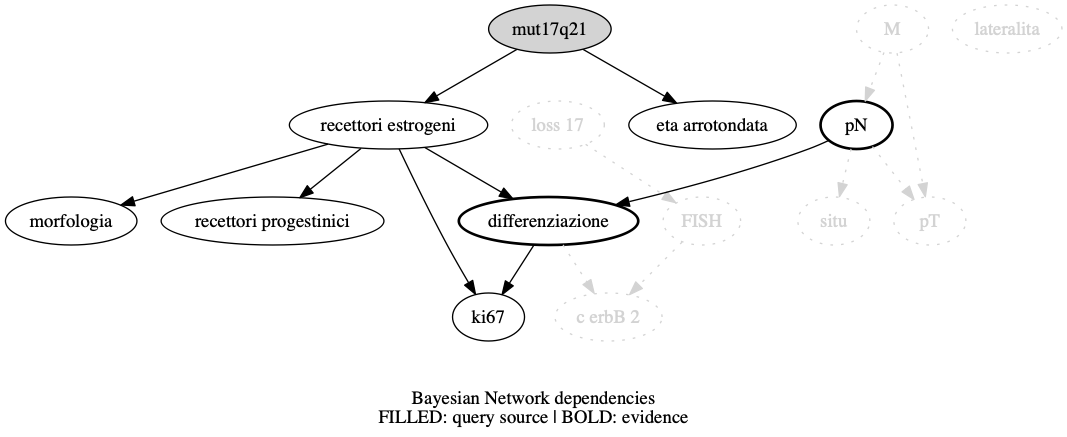
\includegraphics[width=\columnwidth]{methodology/images/d-separation-example}}
\caption{D-Separations in the provided data set (see Sec. \ref{sec:data-set}) generated using the \texttt{plot\_model} function (see Subsec. \ref{subsubsec:plot-model})}
\label{fig:d-separation_example}
\end{figure}


\subsection{Bayesian Networks} \label{subsec:bayesiannetworks}
\begin{definition}
	A Bayesian Network (BN) is a probabilistic graphical model represented by a DAG where each vertex corresponds to a random variable $X_i$ and the edges model the dependencies among these.
\end{definition}
Such a model is basically a way of compactly representing an explicit joint distribution $\mathbb{P}(X_1 \cap \ldots \cap X_n) = \mathbb{P}(X_1) \ldots \mathbb{P}(X_n)$, that is factorised into $\mathbb{P}(X_n \mid X_1 \cap \ldots \cap X_{n-1}) \ldots \mathbb{P}(X_2 \mid X_1 ) \mathbb{P}(X_1) $.
The way this compactness is achieved is in exploiting the independencies that exist among the random variables:
\begin{equation} \label{eq:bnindependencies}
	\forall X_i:  ( X_i \perp \neg Desc(X_i) \mid Pa(X_i))
\end{equation}
with $Pa(X_i)$ the set of nodes that are parents of $X_i$ and $Desc(X_i)$ the nodes that are not \textit{descendents} of $X_i$.
That is to say, every random variable $X_i$, given its parent nodes, is independent of all other nodes in the Bayesian Network that are not descended from it.
Also, a BN gives the flexibility to drop the many weak dependencies that are bound to exist between variables thus leading to an even simpler model.
A full probability table for a joint distribution of random variables obscures the independencies and requires an exponential number of entries for the representation.
A Bayesian Network on the other hand can represent the same distribution using only a linear number of parameters.
The way that Bayesian Networks can be used to reduce the storage requirements for uncertain information is by taking advantage of the conditional independencies embedded in the underlying distribution being modelled.
The power of BNs comes from the additional information encoded in their structure and this was first explicitly described in its entirety by \cite{Pearl1988} who defined the concept of dependence separation (see Subsec. \ref{subsec:d-separation}) and applied it to Bayesian Networks.

One nice characteristic of BNs is that they very naturally model the type of mixed causal and stochastic processes that we find in all of Nature.
Imagine we want to represent the process modelled by joint distribution $\mathbb{P}(B,A) = \mathbb{P}(B) \mathbb{P}(A)$; using the chain rule for conditional probabilities (Eq. \ref{eq:chainrule}) we can write this as $\mathbb{P}(B \mid A) \mathbb{P}(A)$.
A BN modelling this process would be composed of two nodes $A$ and $B$ with an edge from the former to the latter $A \rightarrow B$, $A$ is called the ``parent'' of $B$.  Each of these two nodes would have its own probability table, with $\mathbb{P}(A)$ representing the \textit{prior} distribution over $A$ and $\mathbb{P}(B \mid A)$ the \textit{conditional probability distribution} of $B$ given $A$.

We can now see why these types of models are named \textit{Bayesian} Networks: the inference process is based in a given prior distribution/belief and evolves through a parent $\rightarrow$ child relationship to constantly yield an updated \textit{posterior} belief.
The BN DAG encodes a generative sampling where each variable's value is determined stochastically by Nature, based on the value of its parents.
This process is also highly compatible with our view of causality and this is one of the reason that makes BNs highly interpretable.
The prior $\mathbb{P}(A)$ can be seen as the result of some stochastic process caused by a series of latent (unmodelled) variables while the posterior $\mathbb{P}(B \mid A)$ is stochastically, causally determined by $A$. 
As I have mentioned in the previous paragraphs, there are probably no truly ``prior'' distributions in the Universe, at the modelling scale we are usually interested in.
Only on arriving on the quantum particle level may we find ``pure'' stochastic, uncaused processes due to quantum collapse.

A good example of how BNs are well compatible with our notion of causality may be to imagine $A$ as the random variable modelling the predisposition to having a certain disease and $B$ to actually developing the symptoms for it.
\textit{First}, genetic and epigenetic factors such as the environment stochastically contributed to having the predisposition and \textit{then} the development of the symptoms was stochastically determined by the degree of predisposition.
Adding an extra time dimension certainly helps us in dealing with this class of models.

\subsection{Bayesian Networks Structure Learning} \label{subsec:bnstructurelearning} 
In many probabilistic models initialisation is fast but then fitting the data is slow (ex. k-means).
For Bayesian Networks the converse is true: fitting is fast as only sums of the counts in the data are needed but identifying the correct graph structure can take super-exponential time.
Learning the Bayesian Network structure from data is commonly known as the Bayesian Network Structure Learning (BNSL) problem.
The methods to solve this problem can be roughly categorised into one of three types.

\subsubsection{Search and Score}
This is the most na{\"i}ve method as it does a brute force search over all the possibile graph structure space - i.e. all DAGs with the same number of variables as the input data - and scores all these depending on some cost function.
This process is super-exponential but though the use of dynamic programming and heuristic search algorithms it can become sub-exponential.
Nonetheless, solving the exact BNSL is only feasible up to $~ 30$ variables.

\subsubsection{Constraint Learning}
Methods of this type calculate some measure of correlation to identify the presence and direction of edges between nodes.
A typical test is to iterate over all triplets while testing for conditional independencies.
Thanks to the d-separation properties outlined in Sub-Section. \ref{subsec:bayesiannetworks}, this test is able to identify the correct edges.
The algorithm is quadratic in time in the number of vertices.

\subsubsection{Approximations}
Several heuristical approaches have been developed to be able to find good network structures in an efficient manner.
Examples of these are:
\begin{itemize}
  \item Chow-Liu, that builds a tree approximation of the probability distribution
  \item Greedy hill-climbing, that adds/removes/flips an edge at a time
  \item optimal reinsertion, that iteratively calculates the optimal $Markov blanket$ (the subset of all nodes that are sufficient to determine the value of another subset) of an ever-smaller subset of nodes
\end{itemize}

\subsection{Bayesian Networks Updating} \label{subsec:bnupdating}
All the types of inference presented are instances of \textit{diagnostic reasoning}, also known as \textit{abductive reasoning}.  
This type of explanation can either be modelled as a conditional probability or a MAP query and is of fundamental importance in many important problems of machine learning including medical diagnosis, that is of particular interest to us.

\subsubsection{Conditional Probability Query}
The \textit{updating} problem is the process of updating the probabilities of nodes in the BN based on the observation of the values of other vertices.
This process of conditioning on observed information is also called \textit{data propagation}.

The following algorithm was described by \cite{Normand1992} and applies to our case where the random variables follow a multinomial distribution.
What we want, is to calculate the conditioned probability $\mathbb{P}(B \mid D)$ i.e. the updated probability of node $B$ based on observed evidence $E$.
\begin{definition}
	The conditional probability query for variable $B$ given evidence $E$ is:
\begin{equation} \label{eq:bnupdating}
	\mathbb{P}(B \mid E) = \alpha \pi(B) \lambda(B)
\end{equation}
with $\pi(B) \lambda(B)$ analogous to the \textit{prior} and \textit{likelihood} of $B$, respectively.
\end{definition}
The likelihood of $B$ depends only on the weighted likelihoods of its children $C_1, \ldots ,C_k$:\begin{align}
	\lambda(B) = \prod_l \lambda_{C_l}(B) \\
	\lambda_{C_{l}}(B)=\sum_{C_{l}} \lambda\left(C_{l}\right) P\left(C_{l} \mid B\right)
\end{align}
and its prior similarly depends only on the information received from its parents $A$:
\begin{align}
	\pi(B)=\sum_{A} P(B \mid A) \pi_{B}(A) \\
	\pi_{B}(A)=\alpha \pi(A) \prod_{S_{B}} \lambda_{S_{B}}(A)
\end{align}
The information is propagated down if any variable observed is above $B$ while up if any variable observed lives in the tree rooted in $B$.
Initially all leaf nodes' likelihoods are set at $1$ and the priors of root nodes are assumed to be observable.

\subsubsection{Maximum a Posteriori Query}
Another common type of question we might ask a BN is the following: ``given evidence $E$ which is the most likely assignment of a subset of variables $Y$?''.
This is know as \textit{Maximum a posteriori (MAP)} inference and is a much harder problem that a conditional probability query.
We are trying to solve the an optimisation problem.
\begin{definition}
As defined by \cite{koller2007introduction}.
Given evidence/observed variables $E=e$, $E \subseteq \mathcal{X}$ and sets $Y \subseteq \mathcal{X} - E$ and $Z = \mathcal{X} - E - Y$, with $\mathcal{X}$ the set of all variables in the BN, the MAP query for $Y$ is the assignment of values $Y=y$ that has maximum probability:
	\begin{equation} \label{eq:map}
	\text{MAP}( Y=y \mid E=e ) = \underset{y}{\text{argmax }}  \sum_z \mathbb{P}(Y=y, Z=z \mid E=e)
\end{equation}
\end{definition}


The MAP problem is hard to solve efficiently; that is it is part of the \textit{NP-hard} complexity class, as proved by \cite{Shimony1994}.
Calculating it in a brute-force way would mean elencating all the possible variable-value tuples and computing their joint probabilities; as these are exponential in the number of variables, the problem is evidently untractable.
Moreover, this is true even in a Bayesian Network.  
Such a model may possess a linear number of parameters but the underlying distribution is still exponential.
Explicitly calculating the MAP defeats the very purpose of the BN, that is computational efficiency.
For this reason, there exist a host of approaches to optimising MAP: elimination algorithms, gradient methods, simulated annealing and other stochastic local searches, belief propagation and integer linear programming.

\textbf{A very important thing to note is that the greedy assignment where each variable picks its most likely value can be very different from the most likely joint assignment of all variables.}

\subsubsection{Most Probable Explanation Query}
A special case of MAP is the \textit{Most probable explanation (MPE)} that, 
\begin{definition}
	As defined by \cite{koller2007introduction}.
 Given evidence/observed variables $E=e$, $E \subseteq \mathcal{X}$ and $W = \mathcal{X} - E$, the MPE query for $W$ is the assignment of values $W=w$ that has maximum probability:
	\begin{equation} \label{eq:mpe}
	\text{MPE}( W=w \mid E=e ) = \underset{w}{\text{argmax }} \mathbb{P}(W=w \mid E=e)
\end{equation}
\end{definition}

This is an easier problem than MAP, as can be seen by comparing Eq. \ref{eq:map} with Eq. \ref{eq:mpe}; MAP presents both a summation and a maximisation and as such is part conditional probability query, part MPE query.
All algorithms for the computation of MAP obviously apply to MPE too, but there exist efficient approximate algorithms for MPE that do not generalise to MAP such as Loopy Belief Propagation [\cite{Pearl1988}] and Stochastic Local Search [\cite{Kask1999}].


